%%%%%%%%%%%%%%%%%%%%%%%%%%%%%%%%%%%%%%%%%%%%%%%%%%%%%%%%%%%%%%%%%%%%
%% I, the copyright holder of this work, release this work into the
%% public domain. This applies worldwide. In some countries this may
%% not be legally possible; if so: I grant anyone the right to use
%% this work for any purpose, without any conditions, unless such
%% conditions are required by law.
%%%%%%%%%%%%%%%%%%%%%%%%%%%%%%%%%%%%%%%%%%%%%%%%%%%%%%%%%%%%%%%%%%%%

\documentclass[
  digital, %% The `digital` option enables the default options for the
           %% digital version of a document. Replace with `printed`
           %% to enable the default options for the printed version
           %% of a document.
%%  color,   %% Uncomment these lines (by removing the %% at the
%%           %% beginning) to use color in the printed version of your
%%           %% document
  oneside, %% The `oneside` option enables one-sided typesetting,
           %% which is preferred if you are only going to submit a
           %% digital version of your thesis. Replace with `twoside`
           %% for double-sided typesetting if you are planning to
           %% also print your thesis. For double-sided typesetting,
           %% use at least 120 g/m² paper to prevent show-through.
  lof,     %% The `lof` option prints the List of Figures. Replace
           %% with `nolof` to hide the List of Figures.
  lot,     %% The `lot` option prints the List of Tables. Replace
           %% with `nolot` to hide the List of Tables.
]{fithesis4}
%% The following section sets up the locales used in the thesis.
\usepackage[resetfonts]{cmap} %% We need to load the T2A font encoding
\usepackage{latex-javaScript/jslistings}
\usepackage[T1,T2A]{fontenc}  %% to use the Cyrillic fonts with Russian texts.
\usepackage[
  main=english, %% By using `czech` or `slovak` as the main locale
                %% instead of `english`, you can typeset the thesis
                %% in either Czech or Slovak, respectively.
  english, german, russian, czech, slovak %% The additional keys allow
]{babel}        %% foreign texts to be typeset as follows:
%%
%%   \begin{otherlanguage}{german}  ... \end{otherlanguage}
%%   \begin{otherlanguage}{russian} ... \end{otherlanguage}
%%   \begin{otherlanguage}{czech}   ... \end{otherlanguage}
%%   \begin{otherlanguage}{slovak}  ... \end{otherlanguage}
%%
%% For non-Latin scripts, it may be necessary to load additional
%% fonts:
\usepackage{paratype}
\usepackage{my-alias}
\def\textrussian#1{{\usefont{T2A}{PTSerif-TLF}{m}{rm}#1}}
%%
%% The following section sets up the metadata of the thesis.
\thesissetup{
    date        = \the\year/\the\month/\the\day,
    university  = mu,
    faculty     = fi,
    type        = bc,
    department  = Department of Machine Learning and Data Processing,
    author      = Adam Hlaváček,
    gender      = m,
    advisor     = {RNDr. Vladimír Štill, Ph.D.},
    title       = {Revitalization and Modernization of Web Application of the Epistolary Seminar of Informatics},
    TeXtitle    = {Revitalization and Modernization of Web Application of the Epistolary Seminar of Informatics},
    keywords    = {keyword1, keyword2, ...},
    TeXkeywords = {keyword1, keyword2, \ldots},
    abstract    = {%
      This is the abstract of my thesis, which can

      span multiple paragraphs.
    },
    thanks      = {%
      These are the acknowledgements for my thesis, which can

      span multiple paragraphs.
    },
    bib         = example.bib,
    %% Remove the following line to use the JVS 2018 faculty logo.
    facultyLogo = fithesis-fi,
}
\usepackage{makeidx}      %% The `makeidx` package contains
\makeindex                %% helper commands for index typesetting.
\usepackage[acronym]{glossaries}          %% The `glossaries` package
\renewcommand*\glspostdescription{\hfill} %% contains helper commands
\loadglsentries{example-terms-abbrs.tex}  %% for typesetting glossaries
\makenoidxglossaries                      %% and lists of abbreviations.
%% These additional packages are used within the document:
\usepackage{paralist} %% Compact list environments
\usepackage{amsmath}  %% Mathematics
\usepackage{amsthm}
\usepackage{amsfonts}
\usepackage{url}      %% Hyperlinks
\usepackage{markdown} %% Lightweight markup
\usepackage{listings} %% Source code highlighting
\lstset{
  basicstyle      = \ttfamily,
  identifierstyle = \color{black},
  keywordstyle    = \color{blue},
  keywordstyle    = {[2]\color{cyan}},
  keywordstyle    = {[3]\color{olive}},
  stringstyle     = \color{teal},
  commentstyle    = \itshape\color{magenta},
  breaklines      = true,
}
\usepackage{floatrow} %% Putting captions above tables
\floatsetup[table]{capposition=top}
\usepackage[babel]{csquotes} %% Context-sensitive quotation marks
\begin{document}
%% Uncomment the following lines (by removing the %% at the beginning)
%% and to print out List of Abbreviations and/or Glossary in your
%% document. Titles for these tables can be changed by replacing the
%% titles `Abbreviations` and `Glossary`, respectively.
\clearpage
\printnoidxglossary[title={Abbreviations}, type=\acronymtype]
\printnoidxglossary[title={Glossary}]

%% The \chapter* command can be used to produce unnumbered chapters:
\chapter*{Introduction}
%% Unlike \chapter, \chapter* does not update the headings and does not
%% enter the chapter to the table of contents. I we want correct
%% headings and a table of contents entry, we must add them manually:

\mdstart

The Epistolary Seminar of Informatics (ESI for short) is an annual online competition and also one of the activities of the Faculty of Informatics targeted at high school students. The central part of ESI takes place from September to April in four thematic waves. Each wave consists of at least a dozen tasks in which the participants can learn and then apply various informatics principles. Participants who earn a minimum of 60\% points for completing given tasks awarded throughout all four waves are suitable to be accepted to the Faculty of Informatics without taking entrance exams. Every year ESI has more than five hundred participants that come to solve the tasks on its current website located at https://ksi.fi.muni.cz/.

The current website is created with an outdated framework, and only a fraction of the current organizers have a needed understanding of possible issues. Because of this, the main goal of this thesis is to create a new web application for ESI, while the main focuses of the new application are on easy and effective moderation in terms of long term support.

Secondary goals of this thesis are for the new web application to make the website usable on mobile devices, present older tasks incompatible with the current website and to improve the overall user experience of the web page.

As a part of this thesis, some related modifications are also made to the server part of the ESI infrastructure.

The first two chapters are dedicated to researching other competitions similar to the ESI and their approach to their websites. The third chapter describes the ESI's server-side infrastructure. Chapter 4–6 illustrates the new implementation. Chapter 7 describes the completed application infrastructure. The resulting web application, which is a primary goal of this thesis, can be seen in use at https://ksi.fi.muni.cz/novy-web/.

\end{markdown*}

\markright{\textsc{Introduction}}
\addcontentsline{toc}{chapter}{Introduction}

\mdchap{Current state of the web frontend of Epistolary Seminar of Informatics}

The current web frontend of the Epistolary Seminar of Informatics (ESI for short) was written using the first version of the Ember.js framework. The last minor version of the first version of the Ember.js framework was released on the 12th of June 2015~[@ember-1]. The frontend stayed principally the same throughout the years because the first Ember.js version cannot be upgraded to a more recent and supported version with ease. Following the fact that Ember v1 was released in 2015, present seminar organizers face a few severe issues -- the foremost being security implications of using old and deprecated software and the secondary being the lack of volunteers with enough knowledge of this technology. In its current state, the frontend is singlehandedly managed by Ondřej Borýsek~[@ksi-web-frontend].

Since the support of the utilized framework ended, the organizers have been aware of these issues. They have tried to migrate the used version to a current stable version of Ember, most notably inside a private project called web-frontend-ember3~[@ksi-web-frontend-ember3], but these attempts were not successful. The leading explanation for the prevalence of the current frontend is that all organizers are volunteers. With only a limited time available, the organizers decided to work on more imminent duties. However, this task has gained a significant priority as Ondřej Borýsek will finish his studies shortly, and, consequently, none of the team members will be capable of resolving issues or implementing new features.

When deciding how to approach the development of the new version of the ESI frontend, I was faced with three viable alternatives. The first option was to adapt the web of any similarly focused seminar, which was deemed inappropriate because the ESI frontend has grown its backend with unique features not easily adaptable from other projects. The second possibility was to continue with a previous attempt to upgrade the frontend to the newer version of the Ember framework. This option was also discarded as there is a risk that the project would be eventually hard to manage, similarly to the current state. As per the Stack Overflow 2020 developer survey~[@stackoverflow-survey], the Ember framework is no longer used regularly and thus unsuitable for a long-lasting project.

The last option was to develop a new project from scratch using one of the most used web frameworks. Besides jQuery, which is not a full-featured web framework, the most used ones are React.js and Angular~[@stackoverflow-survey].

React~[@react-github], developed by Meta, is the most popular~[@stackoverflow-survey] full-featured web framework. It is focused on the fast development of responsive web applications while heavily depending on modularity and supporting it via external libraries. This modularity allows the developer to tailor the project's library set precisely for the project's needs. Since component logic in React.js is written in JavaScript instead of templates, it is easy to pass rich data through the applications and keep state out of the DOM~[@reactjs]. An added benefit of React.js is that it is taught on the Faculty of Informatics Masaryk University in a course Modern Markup Languages and Their Applications, which is compulsory for both
Programming and Development~[@fi-pva] program and some specializations of Informatics~[@fi-inf]. Nevertheless, most of the current members of the organizer teams have no experience with web development whatsoever.

Angular~[@angular], developed by Google, on the other hand, includes most of the frequently used features~[@angular-features] like routing, HTTP client, forms manipulation, and internalization. Therefore Angular allows the developers to get familiar with a new project more rapidly without needing to learn about new libraries used within a given project first.

Because the team of seminar organizers changes quite frequently, it is crucial to minimize the entrance barrier for new developers to be capable of modifying the frontend. A lower entrance barrier can be achieved by using a well-established technology with minimal supplementary knowledge required. Concerning precisely that argumentation, Angular was chosen as more fitting and is utilized throughout this thesis.

\end{markdown*}

\mdchap{TODO}

- what is endpoint
- what is frontend
- what is backend
- HTTP methods
- contraction JSON, ESI, API, URL, UX, UI
- docker
- angular modularization
- mastodon
- content policy
- wpa
- ssr
- rxjs
- swagger UI
- good commits
- 0auth
- OSI team, team member lifetime
- other seminars
- bootstrap
- angular.js
- Q \& A


\end{markdown*}

\mdchap{ESI Infrastrucute}

ESI's organizers manage two virtual servers hosted on faculty's Open Nebula platform, both running Debian OS. One of these servers is for production, the second is for testing. Both share the same format - an Apache web server, which server the frontend and reverse proxies the backend.
The production server is called `kleobis` and the development `kyzikos` and I will refer to them troughout this thesis as such.

Kleobis has assigned two domains -- [ksi.fi.muni.cz](https://ksi.fi.muni.cz) for access to the frontend and [rest.ksi.fi.muni.cz](https://rest.ksi.fi.muni.cz) for calling backend endpoints.

Kyzikos has no public access, because it is meant as a development server on which the organizers can test their possibly breaking modification without interfering with the production instance.

The frontend~[@ksi-web-frontend] can be automatically deployed from its repository by building it using GitHub Actions and then copying the built web application on the desired server by calling an automated script on one of the organizers faculty accounts.

The backend~[@ksi-web-backend] has no means for automatic deployment and updating. The process has to be performed manualy, by logging into target server, pulling from the source code repository and performing a manual restart. This is a desired workflow, because updates to the backend server are infrequent and a manual check of functionality after an update increases certanity that the server will work as desired even after the update.

## Backend

The backend server~[@ksi-web-backend] is written as a Python 3 project and acts mainly as a middle-ware between the user and the database. A heavily utilized part of the backend is its capability to execute untrusted code sandboxed, which is a crucial part of the ESI. The backend is also capable of manipulating with a git repository containing data of solvable tasks.

### Code sandboxing

To sandbox untrusted code, mainly originating from participants task evaluations, ESI uses `isolate`~[@isolate] project. This project was developed for the needs of programming contests, so it perfectly fits ESI's needs. It uses so-called boxes, in which an executed command has only a limited, but fully defined, set of capabilies. This can mitigate the risk of overloading the host's system by a program stuck in nevereding loop, using the hosts network as a point of entry for an attacker, or even gaining direct access to the hosts system.

### Python web framework

The ESI backend utilizes the Falcon~[@falcon] framework for handling all HTTP API calls, which is used by companies like PayPal and LinkedIn~[@falcon-usage]. This framework is optimized for creating RESTful~[@rest] API and as such is better suitable for larger volume of incoming requests. Every endpoint is defined as a class, which has an implemented method for every supported HTTP method of this endpoint. This methods are given two parameters -- `request` and `response`. This simplicity of the framework design allows for easy and quick implementation of new endpoints and also for steep learning curve for new project maintainers.

\end{markdown*}

\mdchap{Swagger}

OpenAPI, formerly known as Swagger~[@swagger-about], is a set of projects that together can ease the development process for clients connecting to the exposed backend APIs. This can be achieved by the backend exposing a JSON file documenting the structure of the APIs. This structure mainly includes:

- relative paths to the endpoint inside the application
- expected HTTP method
- expected inputs, which can be inside
    - header
    - parameter
    - form
    - JSON body content
- return code and values

The Swagger also supports advanced features such as defining accepted authorizations means such as API keys or 0auth tokens.

The client that is being implemented against this backend can take use of this information so that it precisely knowns what type of data to send and what type of the data to expect. This makes the development process easier, because it eliminates the possibility of miscommunication between the frontend and backend teams. Every time the API on the backend is changed all that it takes is to regenerate the `swagger.json` file and all the clients can download it and modify their requests according to the new specification.

## swagger-codegen

Another part of the set of OpenAPI projects is a project called `swagger-codegen`~[@swagger-codegen]. This tool is able to parse the `swagger.json` file and produce a code for given language that can be used for manipulating with the backend's API. This is a strong opportunity for the developer as this completely eliminates the need for manually checking how to send a requests, instead all required parameters are passed to a generated function which in turn returns the desired data. Furthermore, when used in conjunction with an explicitly typed language, such as TypeScript, the developer of the client application is immediately notified about an type error when a part of the API changes, allowing for a much faster and more secure development.

Currently, the `swagger-codegen` supports generating code for 40 languages, where a `typescript-angular` and `typescript-fetch` are counted as two distinct languages, even though both use TypeScript as a base.

## swagger-ui

The SmartBear Software also provides a tool called Swagger UI~[@swagger-ui]. This tool was developed to parse the `swagger.json` file and to present it in a easily readable form as a web page. The developer can see every described endpoint with its description, accepted method and expected input and output types. The Swagger UI also provides the possibility to directly call the endpoints from the web page by filling parameters into a form and then examining the result of the API call. The SmartBear Software also presents a [demonstration](https://petstore.swagger.io/#/) of the Swagger UI on its website, which can be used to analyze any `swagger.json` file by providing its URL.

\end{markdown*}


\mdchap{Backend modifications}

## Swagger proxy

### Possible approaches

Because the OSI backend is written with a Python Falkon framework without any specified typing and that request inputs and outputs may span across multiple functions and methods, obtaining this information automatically does not seem as a possible course of action, so the information for the creation of the `swagger.json` file need to be generated from the scratch by manually describing every possible endpoint. It was possible to add the documentation directly to the backend project by using [swaggerit wrapper](https://github.com/dutradda/swaggerit) -- the recommended alternative to a now discontinuied falcon-swagger~[@falcon-swagger], but this approach would require a manual typing of all required fields. Another possibility was to describe the backend API with a TypeScript language by using TypeScript OpenAPI~[@tsoa]. This approach has a significant advantage that it uses a TypeScript interfaces to describe expected inputs and outputs. TypeScript interfaces can also be inherited, making it useful to prevent code duplication and its linked dangers.

### Implemented solution

A new project was created as a part of this thesis, web-backend-swagger~[@ksi-web-backend-swagger]. It uses TypeScript OpenAPI to describe the backend API with a similar file structure to the backend project. 

For comparison, consider following shortened code from the OSI's backend for handling an update request to a forum post:

\newpage
~~~python
class Post(object):
    def on_put(self, req, resp, id):
        if (not req.context['user'].is_org():
            return
        data = json.loads(req.stream.read().decode('utf-8'))['post']
        post = session.query(model.Post).get(id)
        if post is None:
            resp.status = falcon.HTTP_404
            return
        post.author = data['author']
        post.body = data['body']
        req.context['result'] = {'post': util.post.to_json(post, req.context['user'].id)}
~~~


From this code example, it is evident, that the endpoint is expecting a JSON dictionary as an i with a single key `post`, which contains additional dictionary with keys `author` and `body`. This information can be transformed into TypeScript interfaces in a following way:


~~~ JavaScript
export interface PostEdit {
    author: number;
    body: string;
}

export interface PostsEditRequest {
    post: PostEdit;
}
~~~

After examining the response content, it is possible to take use of the TypeScript interface generalization, because the `Post` interface fully includes all parameters from the `PostEdit` interface.

~~~ JavaScript
export interface PostResponse {
    post: Post;
}

export interface Post extends PostEdit {
    id: number,
    thread: number;
    published_at: string;
    reaction: number[];
    is_new: boolean;
}
~~~

With the types of inputs and outputs of the endpoint defined, the endpoint itself can be now defined with TypeScript OpenAPI in a following way:

~~~ JavaScript
// the root path of all enpoints defined inside this class is under /posts/
@Route('posts')
export class EndpointPosts {
// a login is required to access this endpoint
    @Security('ksi')
// this endpoint accepts POST request with a single parameter inside URL path named postId
    @Put('{postsId}')
// this endpoint should be uniquely reffered to as postEditSingle
    public async postsEditSingle(
// the postId parameter inside URL path is a number
        @Path() postsId: number,
// the endpoint expects data of a type PostsEditRequest 
        @Body() postsUpdateRequest: PostsEditRequest,
// this endpoint returns data of a type PostResponse on success
    ): Promise<PostResponse>
    {  /* ... code to process the request ... */  }
~~~

From this information, the TypeScript OpenAPI is able to generate the `swagger.json` endpoint description, which can be visualized by Swagger UI, as seen in figure \ref{fig:swagger-ui}.

\end{markdown*}

\begin{figure}
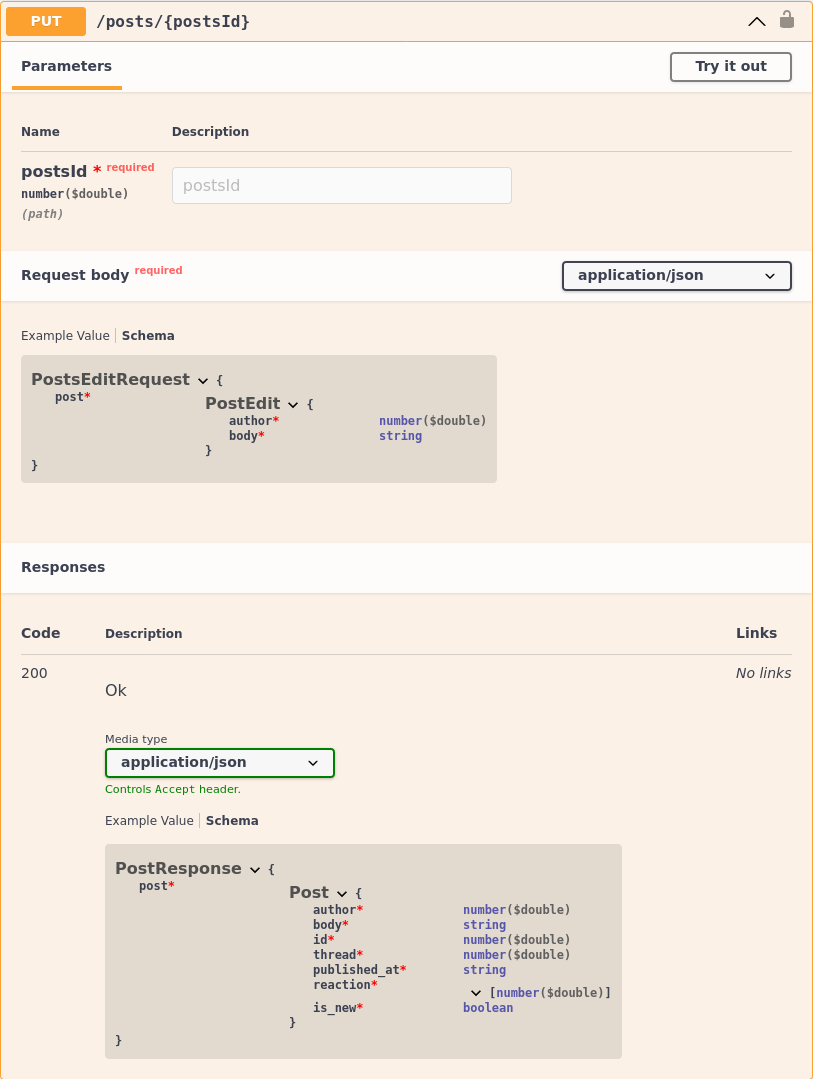
\includegraphics[width=\textwidth]{assets/img/swagger-ui}
\caption{The visualization of the post edit endpoint by Swagger UI}
\label{fig:swagger-ui}
\end{figure}

\mdstart

After the `swagger.json` definition file is generated on the backend, the `swagger-codegen`~[@swagger-codegen] tool can be used to generate respective code on the frontend:

~~~ JavaScript
public postsEditSingle(body: PostsEditRequest, postsId: number): Observable<PostResponse>;
~~~

Internally, this function will take care of handling authorization and possible exceptions, so that the developer can use this as a normal function, without the need to worry about its inner workings.

### Possible drawbacks

Because the definition of the API is stored within a separate project, this could in the future lead to a de-synchronization between the definition of the API and the backend code itself. Though, this threat would be present in some form unless the `swagger.json` can be generated directly from the backend code. If no technology like OpenAPI was used, then the possible issue would move on the client may be updated with less frequency than backend. The separate project is a compromise, which minimizes the risk of de-synchronization by using a simple to use syntax for the backend developers and easy changes implementation by regenerating the code from the Swagger definition for the frontend developers.

\end{markdown*}

\mdchap{Selecting framework for a new web application}

Choosing the right framework, if any, largely impact the structure of the whole application. Because one of the main goals of this thesis is for it to be easily maintainable and quick to understand, the framework must be corresponding to these needs. Given the nature of the composition of the OSI organizers team, where most of the team members do have different skill sets, it is plausible that some of the next maintainers of the OSI web application will have only a basic knowledge about web development in general. Most of this general knowledge is likely to originate from the course PB138 Modern Markup Languages and Their Applications on the Faculty of Informatics Masaryk University. With that in mind, it is evident, that the selected framework needs to be fast to learn and easy to understand with as little background as possible.

## Developing without framework

Even though that it is possible to develop whole application without the use of any existing framework, this approach gains significant problems with the enlarging size of the application. Given that nearly every modern page consist at least of three components -- HTML file defining the elements, JavaScript file with functionality and CSS file used to style the look and placement of elements on the page, it would be possible to import JS and CSS files to different webpages to reuse code. However, this does not apply to HTML, which would have to be a separate file for every web page of the application, resulting in a large reuse of a code. It would be possible to implement a logic that would create complex HTML components from predefined source templates, but this approach would effectively create a new framework. This new framework would then suffer from additional issues like lack of external support and previously untested code.

## Developing with a framework

For reasons shown in the previous section, the development of a larger web application without a framework is not ideal. On the other hand, when a framework is used in the project and then later is the framework marked as obsolete, it can be a challenging task to continue with a maintenance of the project, perhaps best shown on the example of the current OSI web. To select the correct framework for a project, it is possible to investigate the most used ones as they are expected to be supported for a longer period of time. Stack Overflow, a company best known for its site for Q~\&~A regarding computer programming, publishes results of annual survey among developers. According to the 2020 survey~[@stackoverflow-survey] with 36~291 responses from professional developers, the most used web frameworks with at least 25\% of positive responses are jQuery~(43.3\%), React.js~(36.8\%), Angular~(26.5\%). These are the frameworks that I have considered for the new OSI web application.

### jQuery

The jQuery library~[@jquery] is not a full-featured web framework, instead it aims to make common tasks like event handling, animations and document manipulation simpler. As a simple presentation of its capabilities, consider following code with plain JavaScript and jQuery~[@jquery]:

~~~JavaScript
// JavaScript
document.querySelector('button.continue').innerHTML = "Next Step ...";
// jQuery
\$("button.continue").html("Next Step...");
~~~

For its supposed different use case, the jQuery fully lacks advanced features like abstract component creation and styles encapsulation.

### React.js

React~[@reactjs] is a web framework that is being taught on the PB138 Modern Markup Languages and Their Applications course on the Faculty of Informatics Masaryk University. It introduces its own syntax called JSX~[@reactjs-main-concepts]. JSX is a syntax extension of JavaScript, which allows writing HTML template together with JavaScript logic:

~~~JavaScript
function formatName(user) {
  return user.firstName + ' ' + user.lastName;
}
function getGreeting(user) {
  if (user) return <h1>Hello, {formatName(user)}!</h1>;
  else return <h1>Hello, Stranger.</h1>;
}
~~~

The practise of putting JavaSript code and HTML DOM together is useful for the understanding of code by eliminating the need to look on multiple places, possibly split between files. The way of organizing code parts is completely in the hands of the developer.

Main concepts of react are based upon creating components in a form of JavaScript function or ES6 class, which can then be used directly inside the JSX. Component-state management is implemented by saving the state locally and passing functions to child components, which can then propagate events by calling the passed functions as callback. This way of state management, especially when combined with components implemented as functions, makes it possible to produce a cleaner code with well visible dependencies.

The bare React.js without any dependencies does not contain additional features such as CSS encapsulation, meaning that any style defined and imported anywhere in the app will affect even parent components that match its selector, though this feature can be achieved by using the officially supported tool for creating React.js applications.

### Angular
	

\end{markdown*}

\mdchap{Collecting feedback}

## Means of feedback collection

Since the October 2021 the OSI organizers were encouraged to submit their feedback on the state of the new web frontend. The new frontned was scheduled to be made public with a release of the last wave of the OSI year 2021/2022. Up until that date, the organizers have submitted through designated form 9 bug reports and 10 feature suggestions. With the release of the last fourth wave of the OSI year 2021/2022, the feedback was opened also to the participants, together with a questionnaire for them to fill. The participants were motivated to fill the questionnaire by awarding a trophy to everyone who submits it.

## Questionare

The questionare sent to the OSI participants consisted of three parts. In the first part, the participants were asked to provide their opinion on two new experimental UX features. The second section has consisted of questions about comparsion of the new and current OSI web frontend. The last section was made of free form questions about what do participants think that has improved with a new web and what was better on the old web frontend.


\end{markdown*}

\shorthandon{-}

  \printbibliography[heading=bibintoc] %% Print the bibliography.

  \makeatletter\thesis@blocks@clear\makeatother
  \phantomsection %% Print the index and insert it into the
  \addcontentsline{toc}{chapter}{\indexname} %% table of contents.
  \printindex

\appendix %% Start the appendices.
\chapter{An appendix}
Here you can insert the appendices of your thesis.

\end{document}
